In this section, the layer is described in some detail in terms of its specific subsystems. Describe each of the layers and its subsystems in a separate chapter/major subsection of this document. The content of each subsystem description should be similar. Include in this section any special considerations and/or trade-offs considered for the approach you have chosen.

\subsection{Subsystem 1}
This section should be a general description of a particular subsystem for the given layer. For most subsystems, an extract of the architectural block diagram with data flows is useful. This should consist of the subsystem being described and those subsystems with which it communicates.

\begin{figure}[h!]
	\centering
 	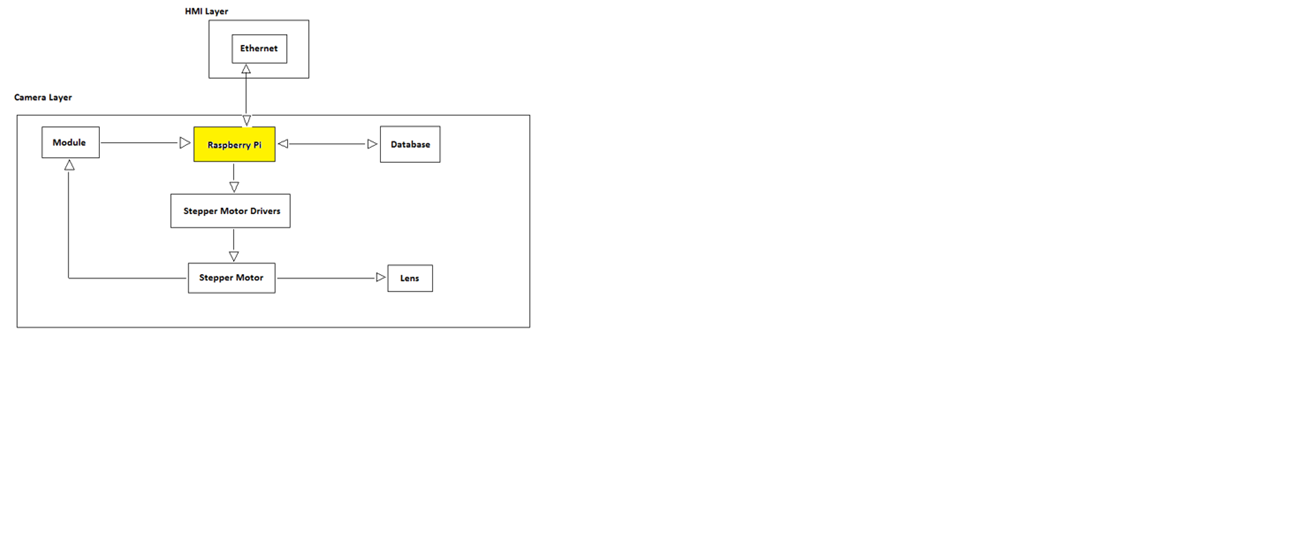
\includegraphics[width=0.60\textwidth]{images/camera_layer.png}
 \caption{Example subsystem description diagram}
\end{figure}

\subsubsection{Assumptions}
The camera layer is assumed to have Ethernet connection and web interface prior to controlling the camera and its movements.  

\subsubsection{Responsibilities}
The camera layer has six subsystems which include Raspberry Pi 2, database, stepper motor drivers, stepper motor, lens, and module. The Raspberry Pi 2 is controlled by user input in the web interface layer, which is then responsible for controlling all other subsystems in the camera layer. The Rpi 2 has Ethernet connection, so all the information sent and received by the Rpi2 is stored in the database, which is used to store logs of important information. The stepper motor driver is essentially software installed on the Rpi2 to control the stepper motors. The stepper motors are connected to the GPIO in the Rpi2 through wires. The lens is responsible for improving camera quality images. The lens is mounted to the stepper motor which moves based on user interaction. The camera module is also controlled by the stepper motor, which moves the camera (pan and tilt) certain degrees based on user interactions.

\subsubsection{Subsystem Interfaces}
Each of the inputs and outputs for the subsystem are defined here. Create a table with an entry for each labelled interface that connects to this subsystem. For each entry, describe any incoming and outgoing data elements will pass through this interface.

\begin {table}[H]
\caption {Subsystem interfaces} 
\begin{center}
    \begin{tabular}{ | p{1cm} | p{6cm} | p{3cm} | p{3cm} |}
    \hline
    ID & Description & Inputs & Outputs \\ \hline
    \#Raspberry Pi & Controls all other subsystems in the camera layer/bus & \pbox{3cm}{ethernet \\ Module} & \pbox{3cm}{Stepper motor drivers \\ database}  \\ \hline
    \#Database & Keep user interaction logs/bus & \pbox{3cm}{Raspberry Pi} & \pbox{3cm}{Raspberry Pi}  \\ \hline
    \#Stepper motor drivers & Allow stepper motor to work/bus & \pbox{3cm}{Raspberry Pi} & \pbox{3cm}{Stepper Motor}  \\ \hline
    \#Stepper motor & Control lens and camera module/bus & \pbox{3cm}{Stepper motor drivers} & \pbox{3cm}{Lens \\ Module}  \\ \hline
    \#Lens & Improve camera quality images/bus & \pbox{3cm}{Stepper motor} & \pbox{3cm}{N/A}  \\ \hline
    \#Module & Take images/bus & \pbox{3cm}{Stepper motor} & \pbox{3cm}{Raspberry Pi}  \\ \hline
    
    \end{tabular}
\end{center}
\end{table}

\subsection{Subsystem 2}
Repeat for each subsystem

\subsection{Subsystem 3}
Repeat for each subsystem

